
\documentclass[a4paper, 12pt]{article}
\usepackage{geometry}
\geometry{margin=2cm}
\usepackage{graphicx} % Required for the inclusion of images
\usepackage[utf8]{inputenc}
%\usepackage{natbib} % Required to change bibliography style to APA
\usepackage{amsmath} % Required for some math elements 
\usepackage[spanish]{babel} 
%\usepackage{fontspec}
\usepackage{lineno,hyperref}
\usepackage{upgreek}
\usepackage{gensymb}
\usepackage{textcomp}
\usepackage{amssymb}
\usepackage{textgreek}
\usepackage{float}
\usepackage{fancyhdr}
\usepackage{dirtytalk}

\allowdisplaybreaks
%\textwidth18cm
%\textheight22cm
%\topmargin0cm
%\oddsidemargin2cm
%\hypersetup{hidelinks}

\usepackage{multirow}

\hypersetup{
    colorlinks=true,
    linkcolor=blue,
    }
\graphicspath{{img}}
\setlength\parindent{0pt} % Removes all indentation from paragraphs

\renewcommand{\labelenumi}{\alph{enumi}.} % Make numbering in the enumerate environment by letter rather than number (e.g. section 6)

\renewcommand{\b}{\textbf}

\newsavebox{\mygraphic}
\sbox{\mygraphic}{
\includegraphics[height=1cm]{logoUNRN.jpg}}


\pagestyle{fancy}

\fancyhead{}

\headheight 16pt

\fancyhead[LO]{\setlength{\unitlength}{1in}
	\begin{picture}(0,0)
		\put(0,0){\usebox{\mygraphic}}
	\end{picture}
	\hspace{1cm}
}

\fancyhead[CO] {\hspace{1.5cm} \large Física I: Ingenierías Ambiental, Electrónica y Telecomunicaciones}

%esto me pareció piola para enumerar los ejercicios
%lo saqué de acá: https://tex.stackexchange.com/questions/302948/numbered-exercises-as-sections
%%%%%%%%%%%%%%%%%%%%%%%%%%%%%%%%%%%%%%%%%5
\newcounter{eje}
\setcounter{eje}{0}
\newcounter{subeje}
\setcounter{subeje}{-1}
\renewcommand\thesubeje{\arabic{eje}\alph{subeje}}%
\newcommand \eje{%
  \vspace{.2cm}
  \par\noindent
  \ifnum\value{subeje}>-1
    \refstepcounter{subeje}%
    \llap{\thesubeje)\quad}%
  \else
    \refstepcounter{eje}%
    \llap{\theeje)\quad}%
  \fi
}
\begin{document}
\pagestyle{fancy}

\begin{center}

	{\Large \textbf{Práctica 2a}}
 
\vspace{.2cm}

{Estática}
\end{center}

\eje  [p.35] Hallar la tensión en cada una de las cuerdas de una estructura ideada por el viejito de
Newton para sostener su manzana, la que pesa unos 200 N (es una manzana importante).

\begin{figure}[H]
\begin{center}
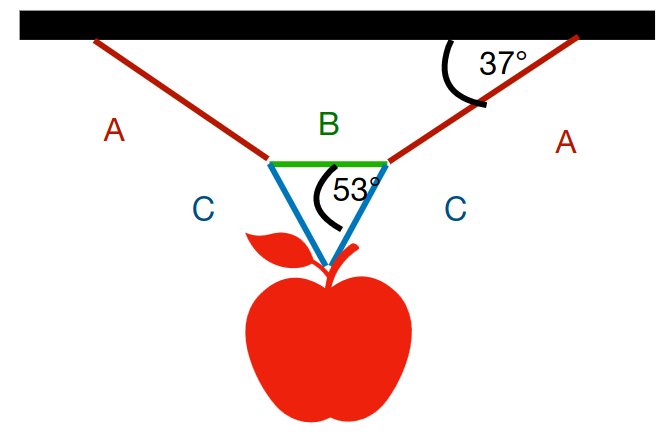
\includegraphics[clip,width = .45\columnwidth]{2af1}
\end{center}
\end{figure}

\eje [4.10] Un bloque de masa m = 2.0 kg es sostenido en equilibrio sobre un plano inclinado que
forma 60° con la horizontal, como indica la figura.

a) Determine el valor de la fuerza \b F;

b) determine la fuerza normal ejercida por el plano inclinado sobre el bloque (ignore la fricción).
\begin{figure}[H]
\begin{center}
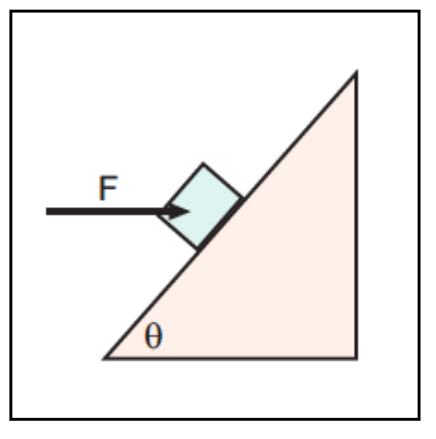
\includegraphics[clip,width = .45\columnwidth]{2af2}
\end{center}
\end{figure}

\eje [4.11] Un bloque de masa m$_1$ = 3.70 kg, sobre un plano inclinado sin fricción a 30° de la
horizontal, está conectado por medio de una polea (sin masa y la que tampoco ejerce fricción) a
un segundo bloque de masa m$_2$ = 2.30 kg, el que cuelga verticalmente como lo muestra la figura.

a) Determine la magnitud de la aceleración de cada bloque;

b) indique hacia dónde se mueve la segunda masa;

c) calcule la tensión de la cuerda.

\begin{figure}[H]
\begin{center}
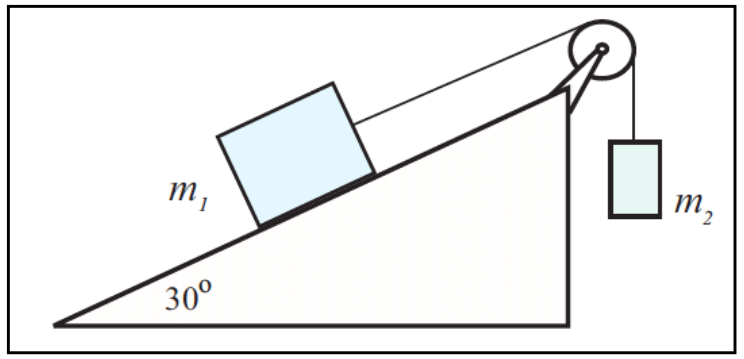
\includegraphics[clip,width = .45\columnwidth]{2af3}
\end{center}
\end{figure}

\eje [4.13] Una masa M está sostenida por una fuerza \b F y un sistema de poleas como se muestra en la
figura. Considere que la polea no tiene fricción ni masa. Entonces, encuentre:

a) las tensiones en cada sección de la cuerda (\b T$_{1,2,3,4,5}$) y

 b) la magnitud de \b F

\begin{figure}[H]
\begin{center}
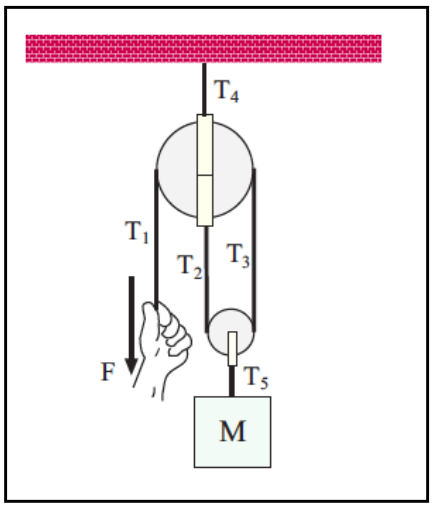
\includegraphics[clip,width = .45\columnwidth]{2af4}
\end{center}
\end{figure}

\eje [5.2] El bloque B de la figura pesa 711 N. El coeficiente de fricción estática entre el bloque y la
mesa es de 0.25. Asuma que la cuerda entre el bloque y el nudo es horizontal. Encuentre,
entonces, el peso máximo del bloque A para el cual el sistema se mantendrá en reposo.


\begin{figure}[H]
\begin{center}
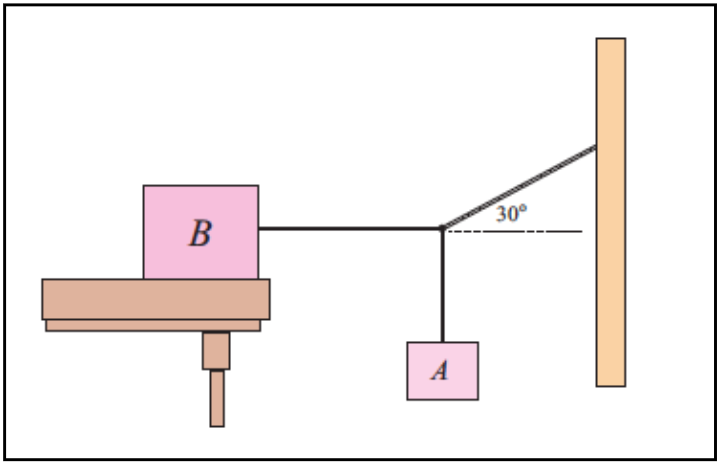
\includegraphics[clip,width = .45\columnwidth]{2af5}
\end{center}
\end{figure}
\end{document}